\documentclass[border=10pt]{standalone}
\usepackage{pgfplots}
\pgfplotsset{compat=1.8}
\begin{document}
\pgfplotsset{colormap={CM}{color=(white) color=(gray!50) color=(gray)}}
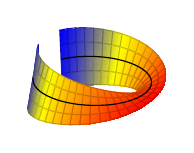
\begin{tikzpicture}
  \begin{axis}[width=4cm,
    hide axis,
    view = {40}{40}
  ]
  \addplot3 [
    surf,
    shader     = faceted interp,
    point meta = x,
    samples    = 40,
    samples y  = 5,
    z buffer   = sort,
    domain     = -160:160,
    y domain   =-0.5:0.5
  ] (
    {(1+0.5*y*cos(x/2)))*cos(x)},
    {(1+0.5*y*cos(x/2)))*sin(x)},
    {0.5*y*sin(x/2)}
  );

  \addplot3 [
    samples=50,
    domain=-145:160, % The domain needs to be adjusted manually,
                     % depending on the camera angle, unfortunately
    samples y=0,
  ] (
    {cos(x)},
    {sin(x)},
    {0}
  );
  \end{axis}
\end{tikzpicture}
\end{document}
